\section{Durchführung}
\subsection{Theoretischer Teil}

\subsection{Kalibriermessungen}
    \subsubsection{Messung einer Quelle bekannter Aktivität bei mittiger Quellposition}
       Zunächst haben wir eine Quelle in mittigem Abstand zu den beiden Detektoren vermessen. Die Quelle hatte am 29.10.2015 eine Aktivitiät $A = \unit[1,02]{MBq}$.\\
       \vspace{2mm}
        
       \begin{tabular}{p{6cm}p{6cm}l}
               \minipanf 
                   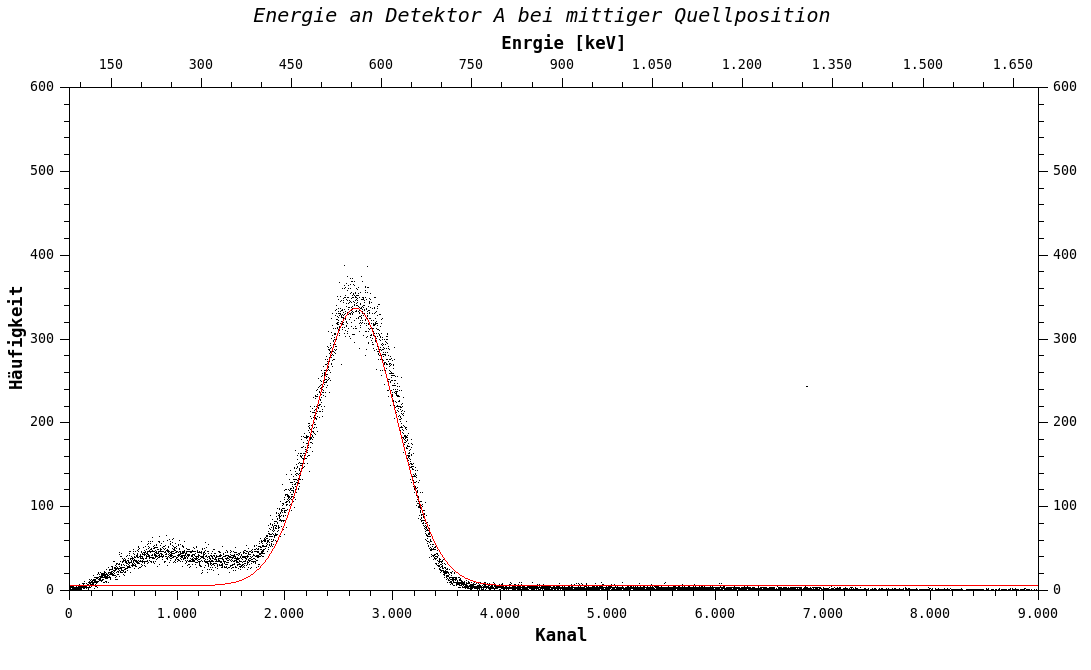
\includegraphics[width=1.2\textwidth, height=0.225\textheight]{pic/Efenster_DetA_M.png}
                   \label{dfd:EdetA_M}
               \minipend
               &
               \hspace{9mm}
               \minipanf 
                   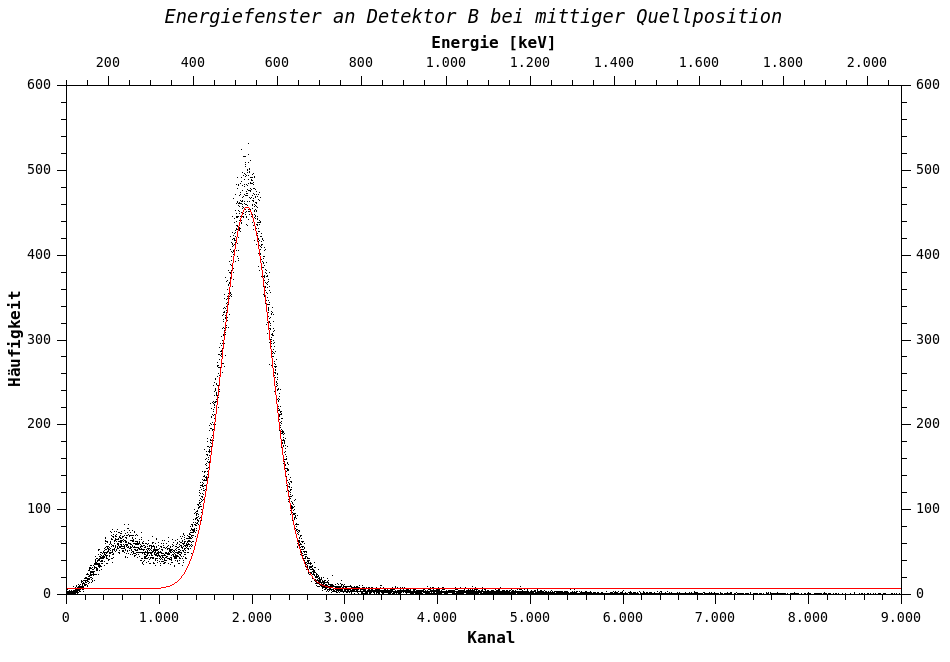
\includegraphics[width=1.2\textwidth, height=0.225\textheight]{pic/Efenster_DetB_M.png}
                   \label{dfd:EdetB_M}
               \minipend\\
               \multicolumn{2}{c}{\hspace{1.5cm}
                   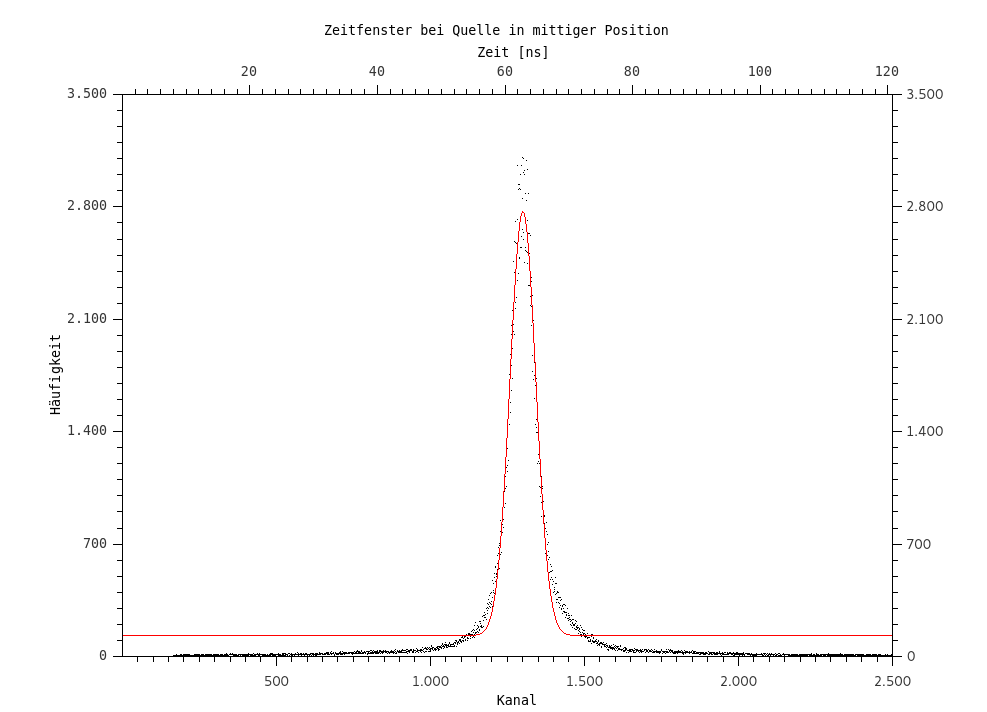
\includegraphics[width=0.7\textwidth, height=0.3\textheight]{pic/T_M_dia.png}
                   \label{dfd:T_M}}\\                        
       \end{tabular}
       \captionof{figure}{Kalibrationsmessung bei Quelle mittig zwischen den Detektoren A und B}


    \subsubsection{Messung bei Positionen direkt an den Detektoren}
        \begin{tabular}{p{6cm}p{6cm}l}
            \minipanf 
                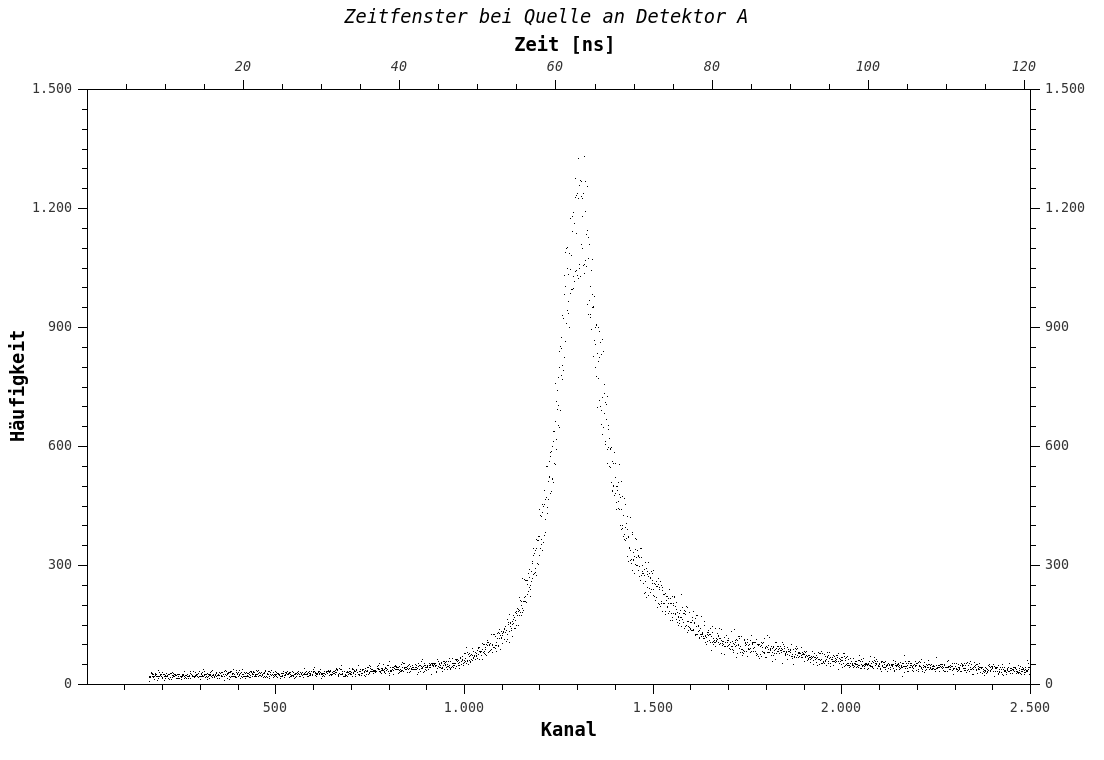
\includegraphics[width=1.2\textwidth, height=0.225\textheight]{pic/T_A_dia.png}
                \label{dfd:T_A}
            \minipend
            &
            \hspace{9mm} 
            \minipanf
                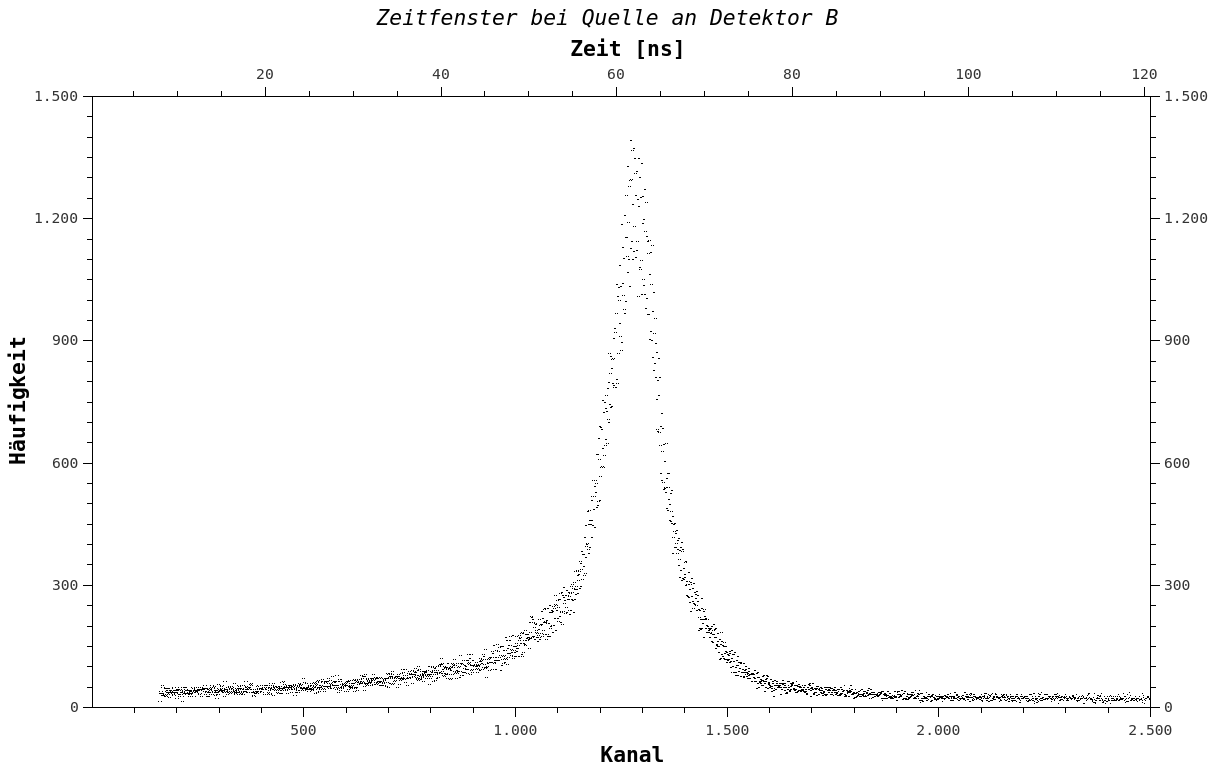
\includegraphics[width=1.2\textwidth, height=0.225\textheight]{pic/T_B_dia.png}
                \label{dfd:T_B}
            \minipend \\
            \minipanf
                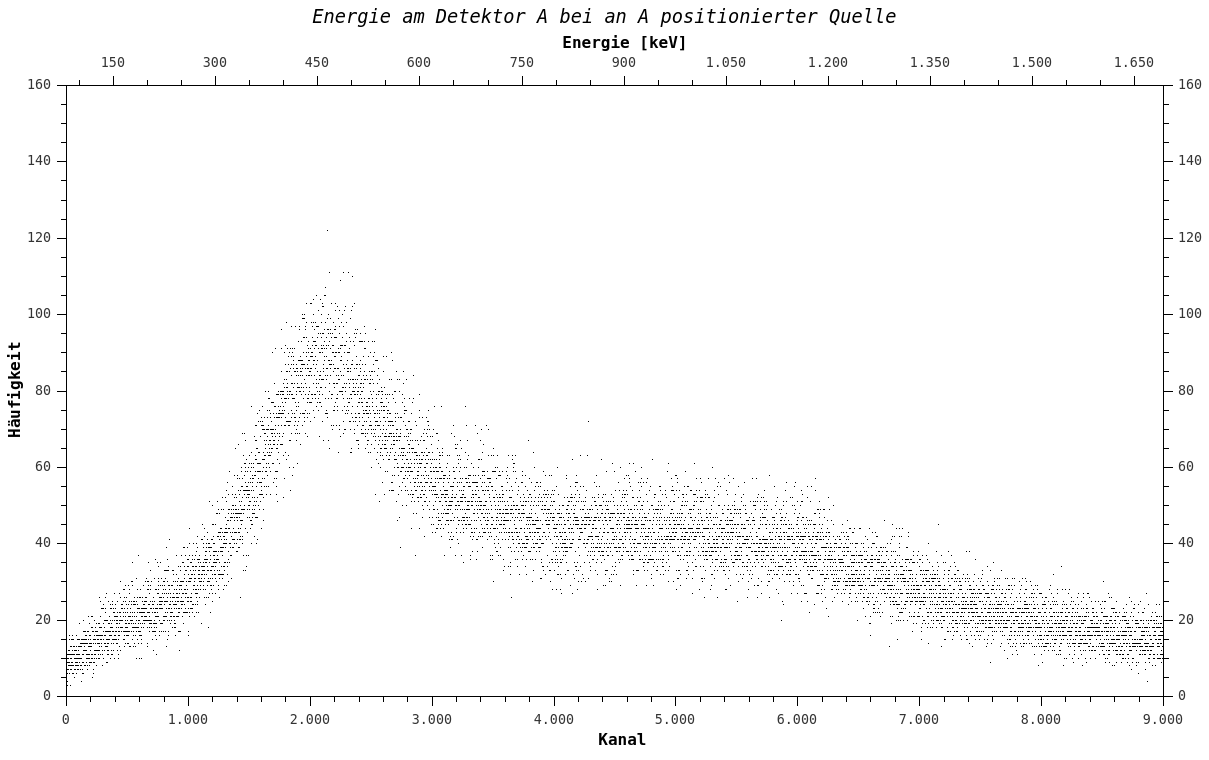
\includegraphics[width=1.2\textwidth, height=0.225\textheight]{pic/Efenster_DetA_A.png}
                \label{dfd:EdetAA}
            \minipend
            &
            \hspace{9mm} 
            \minipanf 
                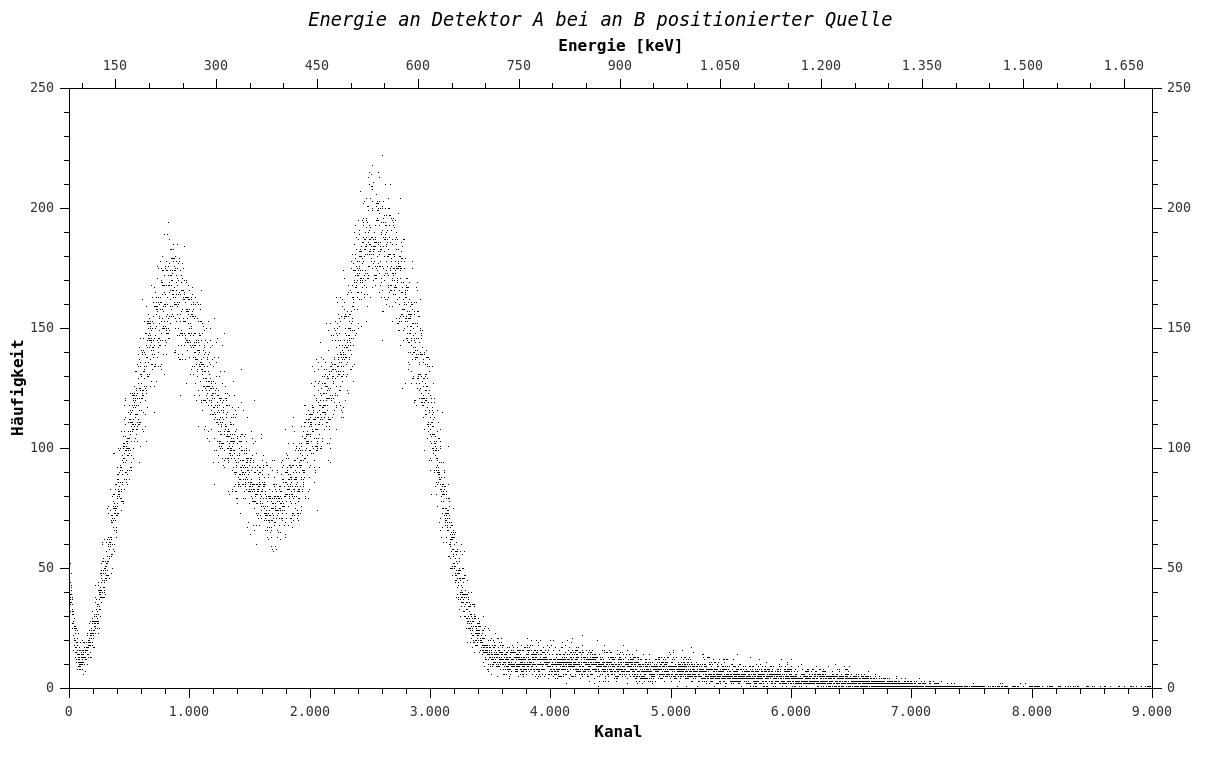
\includegraphics[width=1.2\textwidth, height=0.225\textheight]{pic/Efenster_DetA_B.png}
                \label{dfd:EdetBA}
            \minipend \\
            \minipanf 
                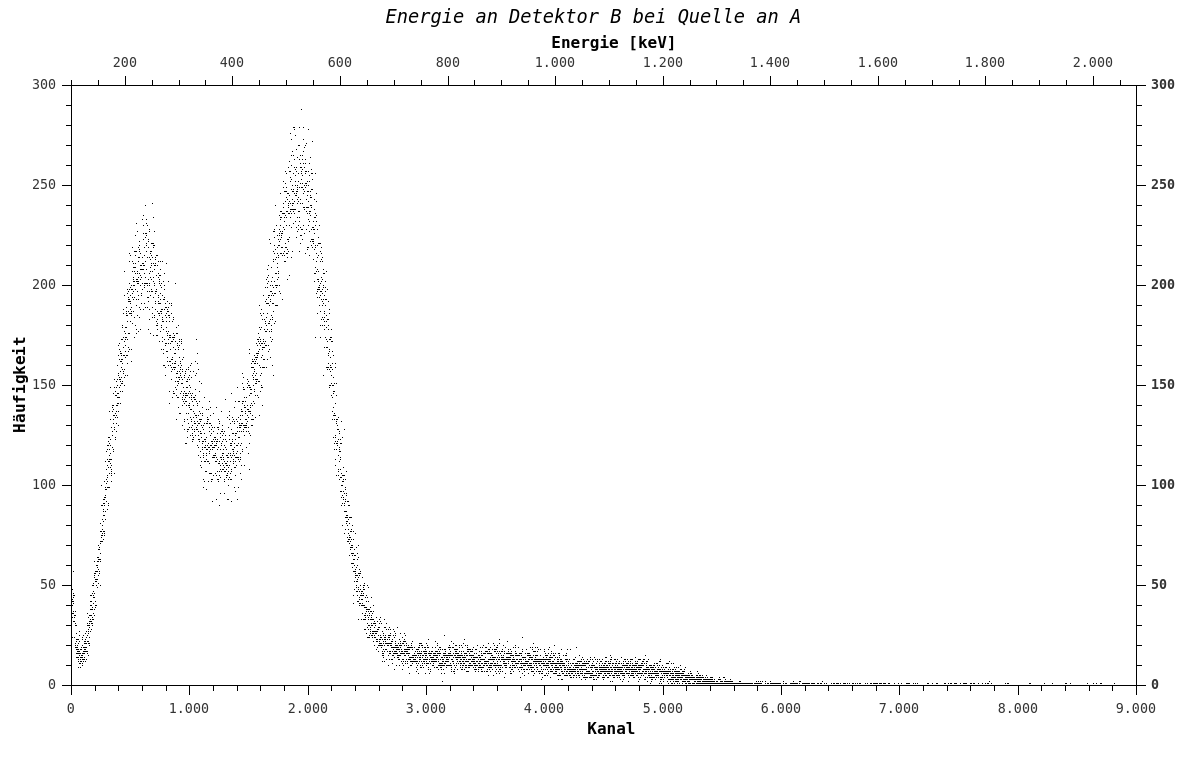
\includegraphics[width=1.2\textwidth, height=0.225\textheight]{pic/Efenster_DetB_A.png}
                \label{dfd:EdetAB}
            \minipend
            &
            \minipanf 
                \hspace{9mm}
                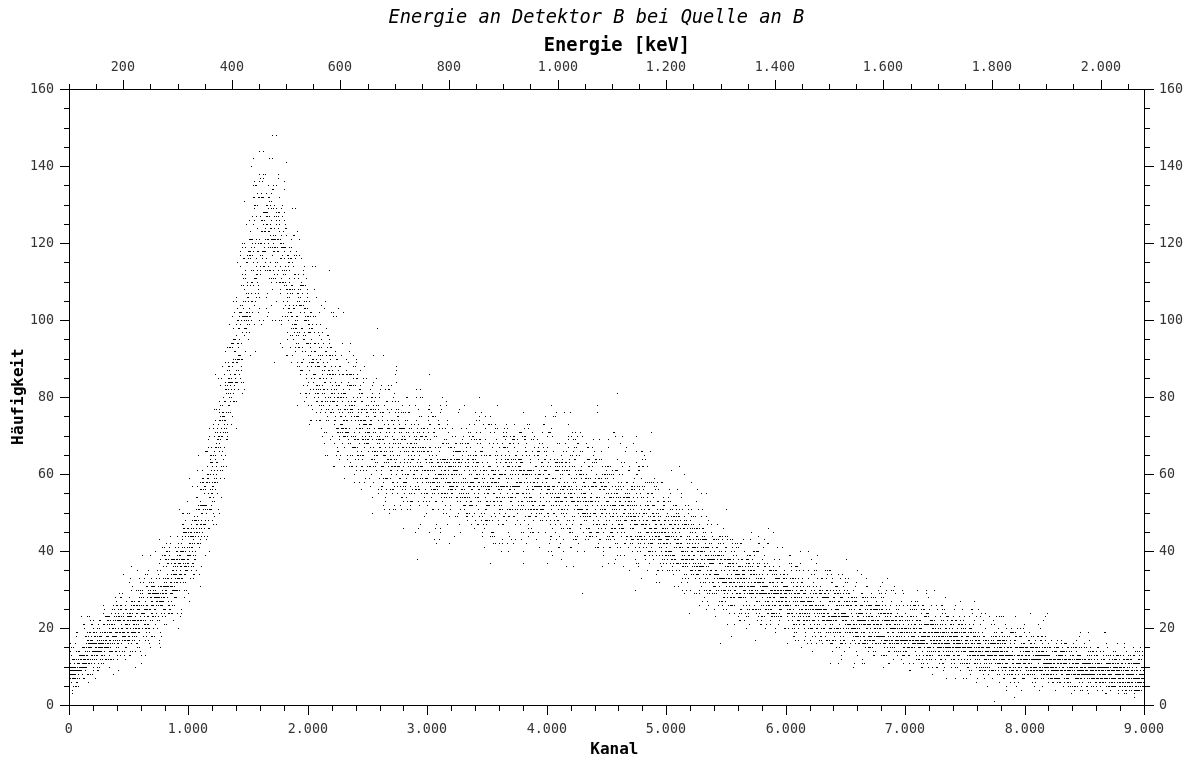
\includegraphics[width=1.2\textwidth, height=0.225\textheight]{pic/Efenster_DetB_B.png}
                \label{dfd:EdetBB}
            \minipend \\            
        \end{tabular}
        \captionof{figure}{Gegenüberstellung der Messungen mit der Quelle an Det. A (links) und Det. B (rechts)} 
        
    \subsection{Tomografische Messungen}
    	\subsubsection{Messung einer Quellkonfiguration, Phantom isotroper Dichteverteilung}
            \textbf{Hauptversuch}\\
            \begin{tabular}{p{6cm}p{6cm}l}
                \minipanf 
                    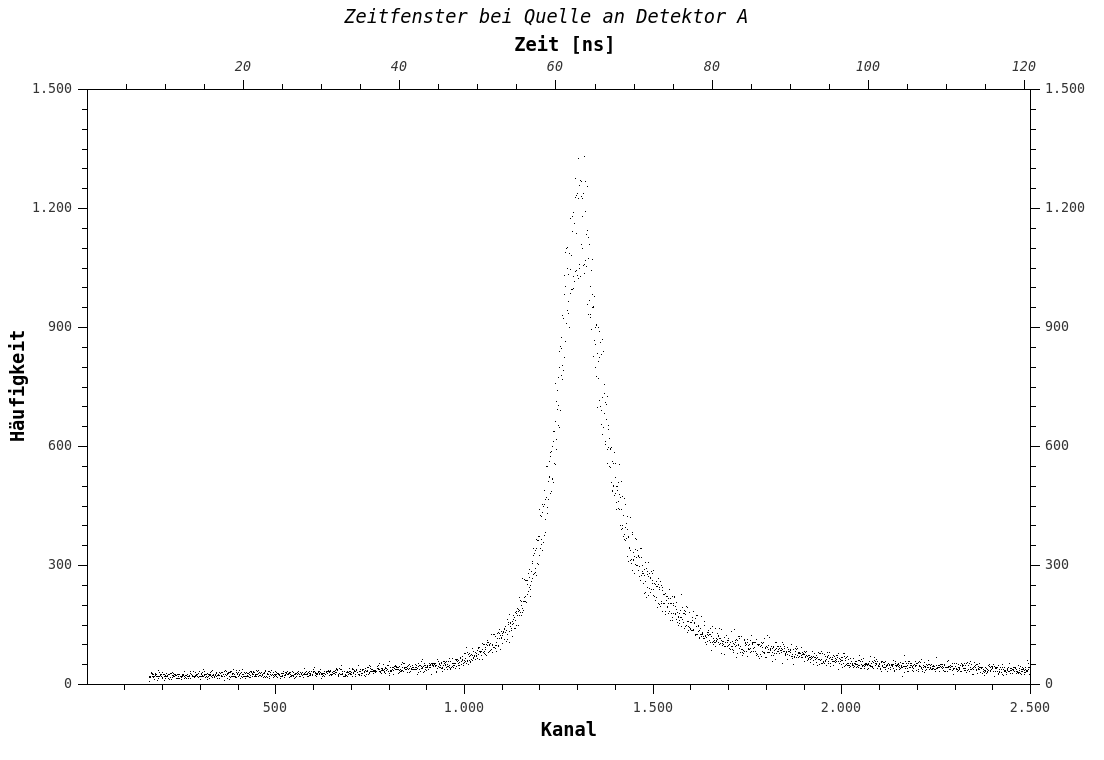
\includegraphics[width=1.2\textwidth, height=0.225\textheight]{pic/T_A_dia.png}
                    %\label{dfd:T_A}
                \minipend
                &
                \hspace{9mm} 
                \minipanf
                    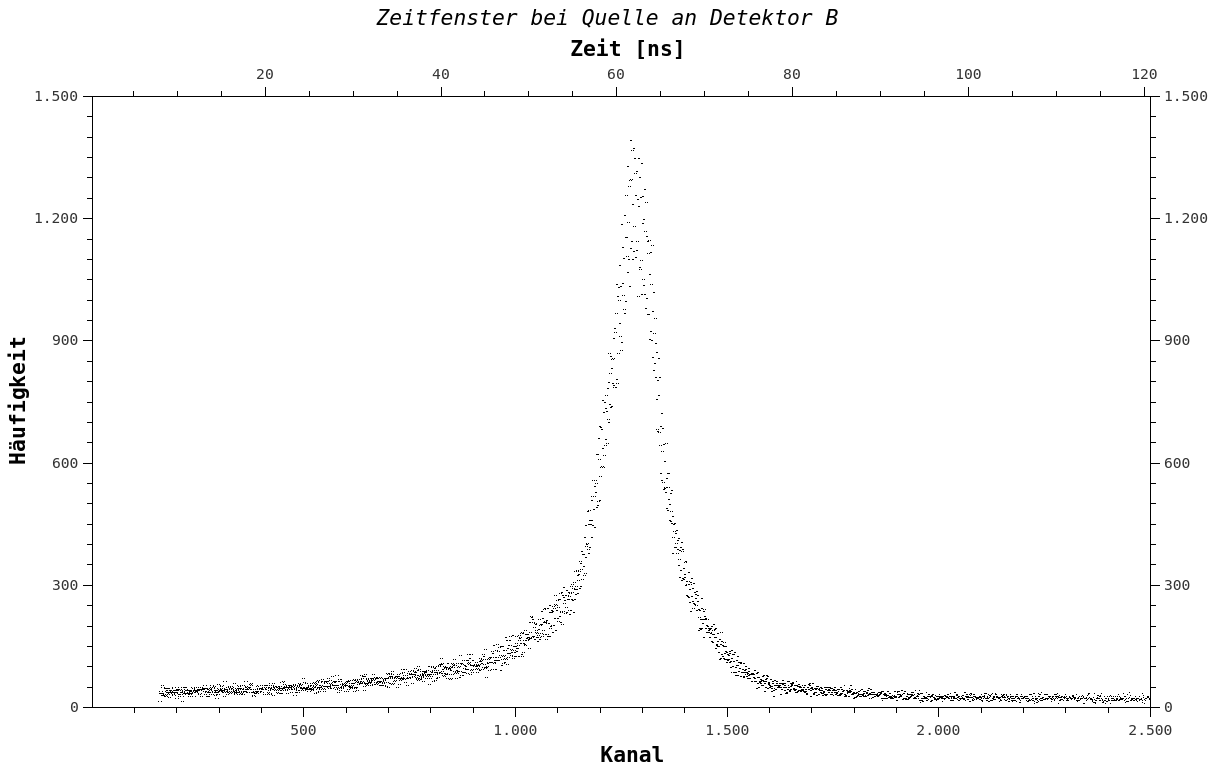
\includegraphics[width=1.2\textwidth, height=0.225\textheight]{pic/T_B_dia.png}
                    %\label{dfd:T_B}
                \minipend \\               
            \end{tabular}
            
            \textbf{Untersuchung des Einflusses verschiedener Filter}\\
            
            \begin{tabular}{p{6cm}p{6cm}c}
                            \minipanf 
                                \makebox[\linewidth]{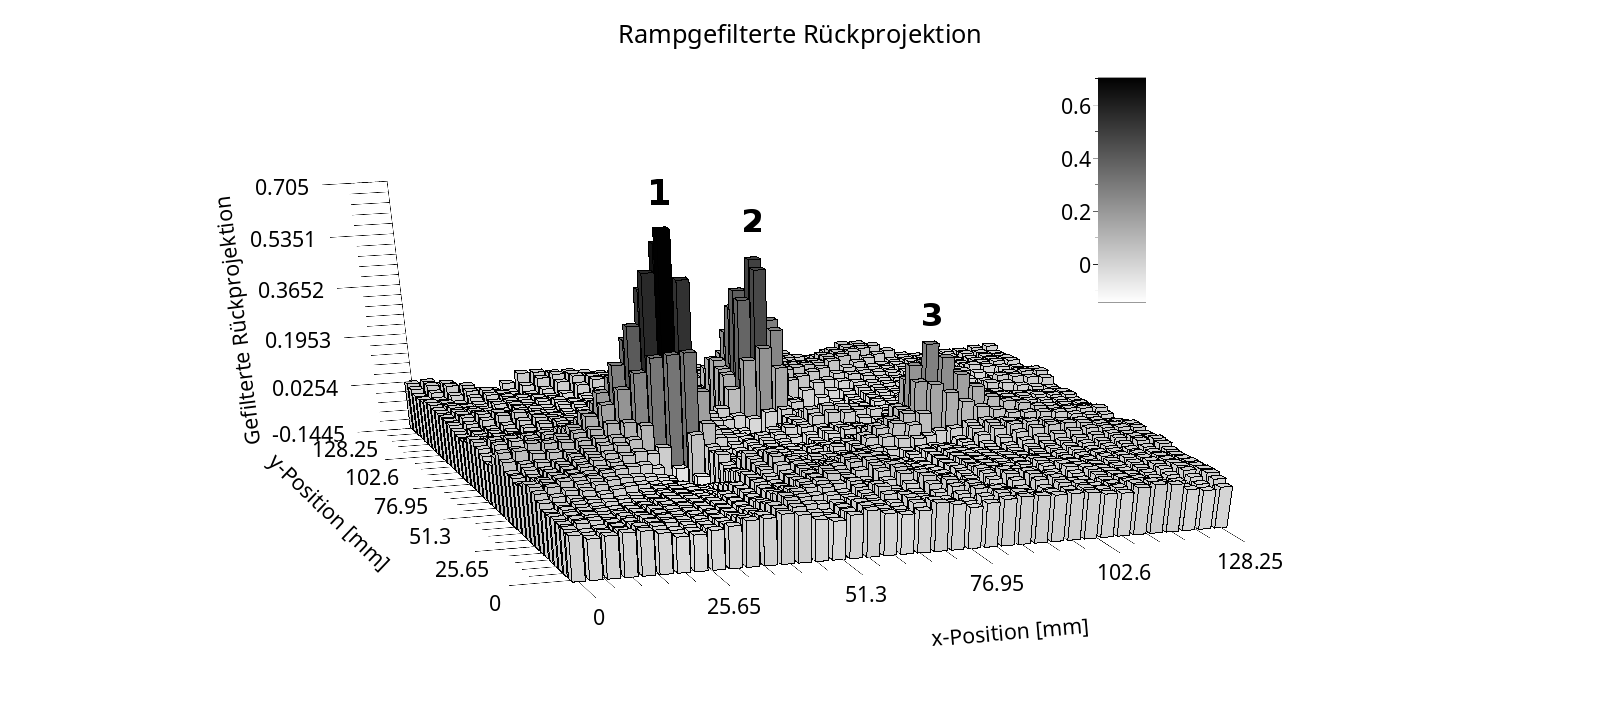
\includegraphics[width=2\textwidth, height=0.225\textheight]{pic/3dPlotTomographRamp.png}}
                                
                            \minipend
                            &
                            \hspace{3mm} 
                            \minipanf
                                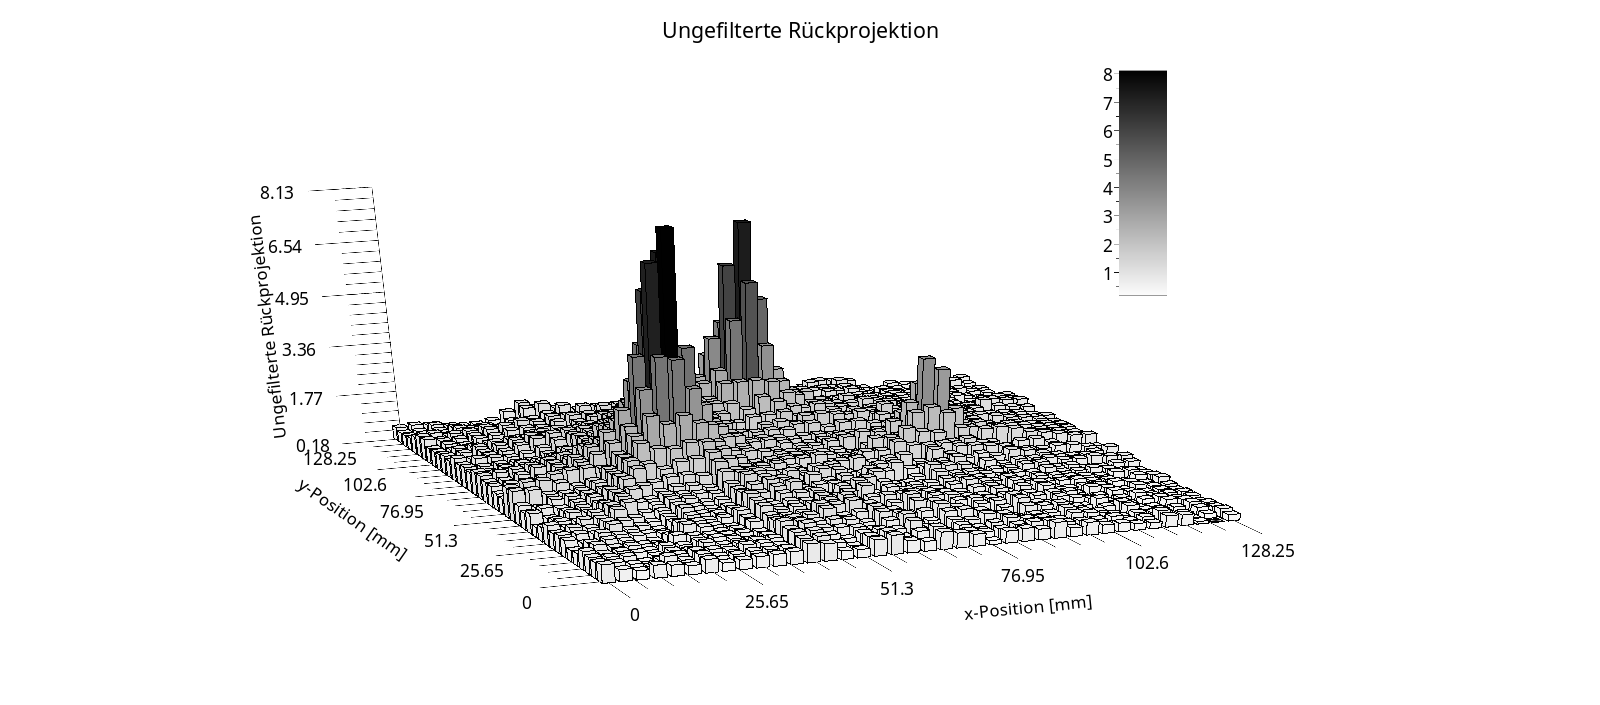
\includegraphics[width=2.2\textwidth, height=0.25\textheight]{pic/3dPlotTomographUngef.png}
                            \minipend \\               
             
             \end{tabular} 
            \captionof{figure}{Gefilterte und Ungefilterte Rückprojektion der Aktivitätsverteilung}
            \label{dfd:AKV}
            \ \\
            
            \textbf{Quantitative Auswertung}
            
            \begin{tabular}{p{12cm}	p{0.5\textwidth}}            	
            	\minipanf
            		Zunächst werden die Positionen $(x_i,y_i) (i = 1,2,3)$ der 3 Quellen im verschlossenen Plastikbehältnis bestimmt. Dafür wird die in Abbildung (\ref{dfd:AKV}) visualisierte Rückprojektion $N(x,y)$ verwendet, die durch Auslesen der in \texttt{Matrix\_reco.txt} enthaltenen Messwertmatrix entstanden ist. Der erste Eintrag sei als Koordinatenursprung gewählt. 1 BIN des Rekonstruktionsrasters entspricht $3,375\ \unit{mm}$. Die Positionen der Quellen werden mit den lokalen Maxima $N(x_i,y_i)$ der Aktivitätsverteilung identifiziert.\\
            		Anschließend quantifiziert man die Aktivität jeder einzelnen Quelle, indem man die rückprojizierten Verteilung über einen kleinen Bereich um die Peaks mittelt. Bezeichne diesen Mittelwert mit $\bar{N}(x_i,y_i)$. Im Rahmen dieser Auswertung wurde ein quadratischer Bereich gewählt, in welchem Werte anzutreffen waren, die in der Nähe des FWHM (=Full Width Half Maximum) lagen. Dieses Vorgehen wird durch die nebenstehende Abbildung visualisiert.
            	\minipend            
            	&
            	\begin{minipage}[c]{\textwidth}
                	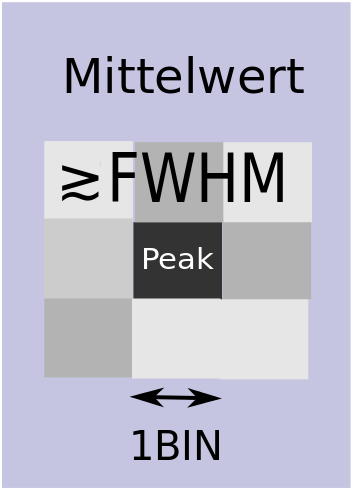
\includegraphics[width=0.35\textwidth, height=0.3\textheight]{pic/Skizze_Mittelung.png}
                \end{minipage}
            \end{tabular}
            
            Mittels einfacher Verhältnisbildung können unter Vorgabe einer Referenzaktivität $A_{ref}$ nun unbekannte Aktivitäten innerhalb der Verteilung berechnet werden. Dabei wurde die stärkste Aktivität mit $A_0 \equiv A(t_0 = \textrm{01.02.2010}) = (363 \pm 11)\ \unit{kBq}$ angegeben. Mit dem Aktivitätsgesetz kann man nun berechnen:
            
            \begin{equation}
            	A_{ref} \equiv A(t =\textrm{29.10.2015}) = A_0 \cdot \left( \frac{1}{2}\right)^{\frac{t-t_0}{T_{1/2}}} = (79 \pm 3)\ \unit{kBq}
            \end{equation}\\
            Wobei die Halbwertszeit $T_{1/2}(^{22}\textrm{Na}) = (2,6027 \pm 0,0010)\ \unit{a}$ verwendet wurde, sowie folgende Fehlerformel:
            \begin{equation}
                \left(\frac{\Delta A_{ref}}{A_{ref}}\right)^2 = \left(\frac{\Delta A_0}{A_0}\right)^2 + \left(\ln(2) \cdot \frac{\Delta T_{1/2}}{T_{1/2}}\right)^2
            \end{equation}\\   
            Bezeichnet man $A_{ref} \propto \bar{N}_{ref} \equiv \bar{N}(x_1,y_1)$ als rückprojizierte Aktivität der Referenzquelle, so erhält man für die unbekannten Aktivitäten $A_i \propto \bar{N}(x_i,y_i)$:
            \begin{equation}
            	A_i = A_{ref} \cdot \frac{\bar{N}(x_i,y_i)}{\bar{N}_{ref}}
            \end{equation}    
            \begin{equation}
                 \left(\frac{\Delta A_i}{A_i}\right)^2 = \left(\frac{\Delta A_{ref}}{A_{ref}}\right)^2 + \left(\frac{\Delta \bar{N}(x_i,y_i)}{\bar{N}(x_i,y_i)}\right)^2 + \left(\frac{\Delta \bar{N}_{ref}}{\bar{N}_{ref}}\right)^2
             \end{equation}\\   
             Hierbei wurden die Fehler der rückprojizierten Aktivitäten als Standardabweichungen des Mittelwertes gesetzt, die sich beim obigen Mittelvorgang ergab: $\Delta \bar{N}(x_i,y_i) = \sigma(\bar{N})$. Die systematischen Fehler des PET-Scanners waren leider nicht bekannt. Zusammenfassend ergeben sich folgende Resultate:  
            
        \subsubsection{Messung einer Quellkonfiguration, Phantom isotroper Dichteverteilung}
          \textbf{Hauptversuch}\\
             \ \\
          Als nächsten wurde eine Messung mit unbekannter Quellverteilung gestartet. Die Energie- und das Zeitfenster entsprechen den oben bestimmten Intervallen.
          \minipanf  
            \begin{center}
            \begin{tabular}{p{7cm}p{7cm}c}
                ungefilterter Projektion & gefilterte Rückprpjektion\\
                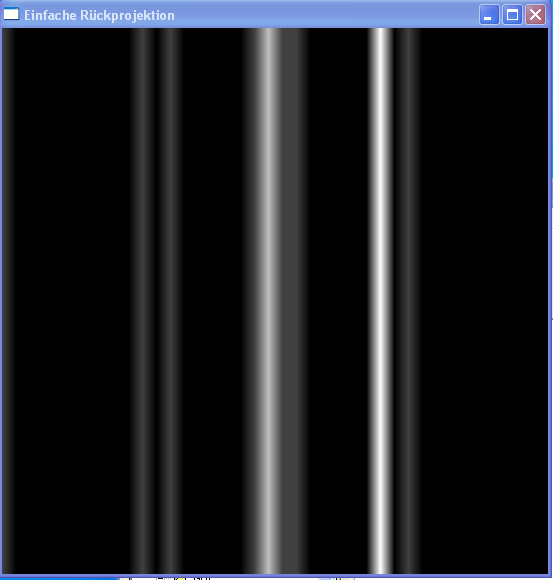
\includegraphics[width=0.3\textwidth, height=0.2\textheight]{pic/Einzelfenster_Bilder/unbekannte_Quelle/unbek1_einf_prj.png}
                & 
                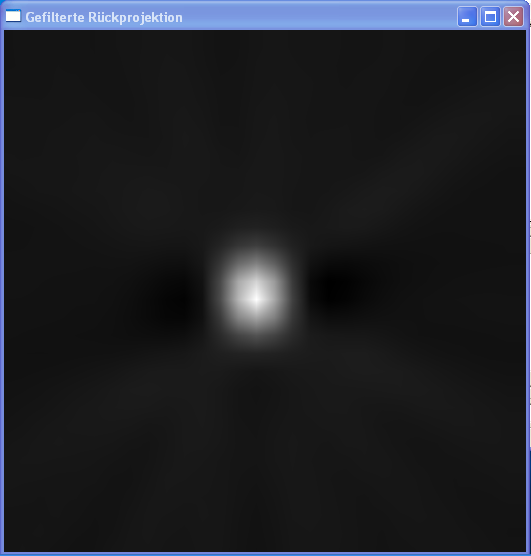
\includegraphics[width=.3\textwidth, height=0.2\textheight]{pic/Einzelfenster_Bilder/unbekannte_Quelle/unbek1gef_prj.png}\\
                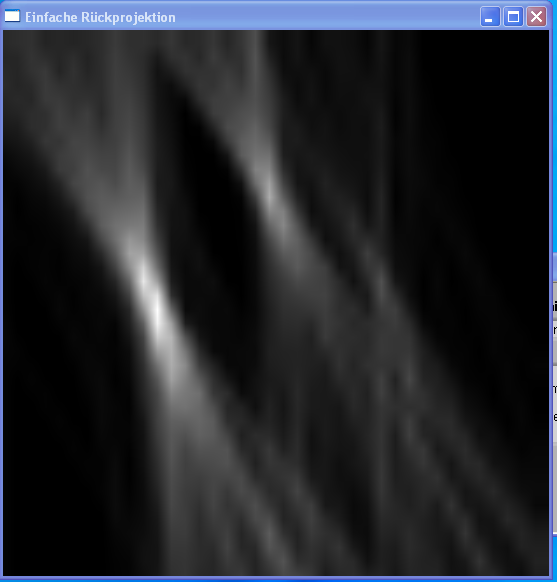
\includegraphics[width=0.3\textwidth, height=0.2\textheight]{pic/Einzelfenster_Bilder/unbekannte_Quelle/unbek2einf_prj.png}
                & 
                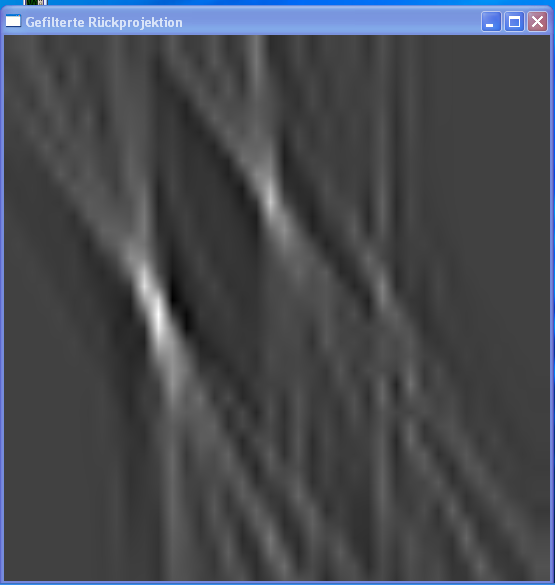
\includegraphics[width=.3\textwidth, height=0.2\textheight]{pic/Einzelfenster_Bilder/unbekannte_Quelle/unbek2gef_prj.png}\\ 
                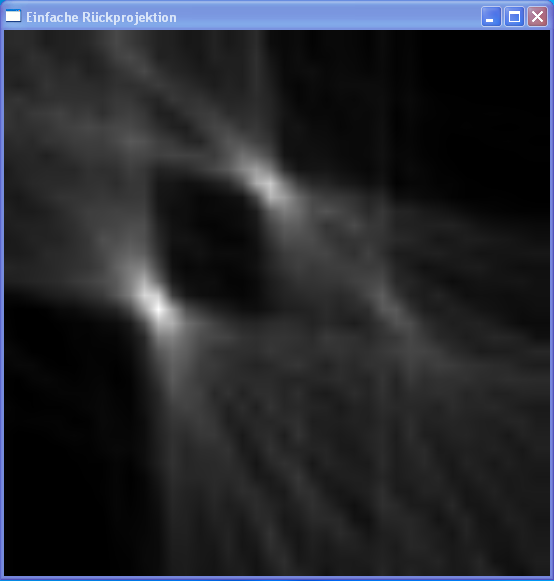
\includegraphics[width=0.3\textwidth, height=0.2\textheight]{pic/Einzelfenster_Bilder/unbekannte_Quelle/unbek3einf_prj.png}
                & 
                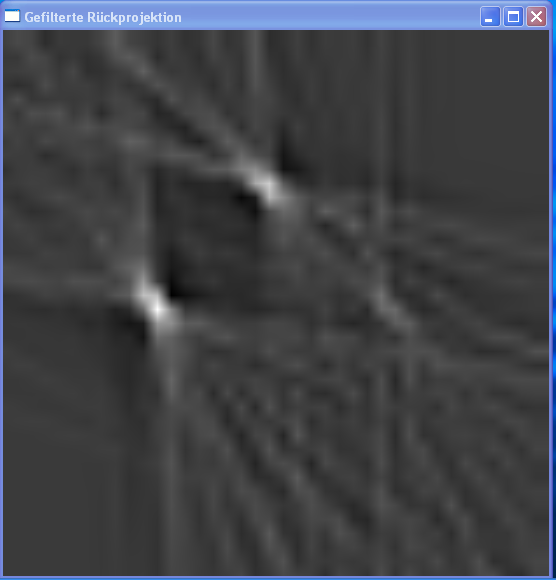
\includegraphics[width=.3\textwidth, height=0.2\textheight]{pic/Einzelfenster_Bilder/unbekannte_Quelle/unbek3gef_prj.png}\\               
                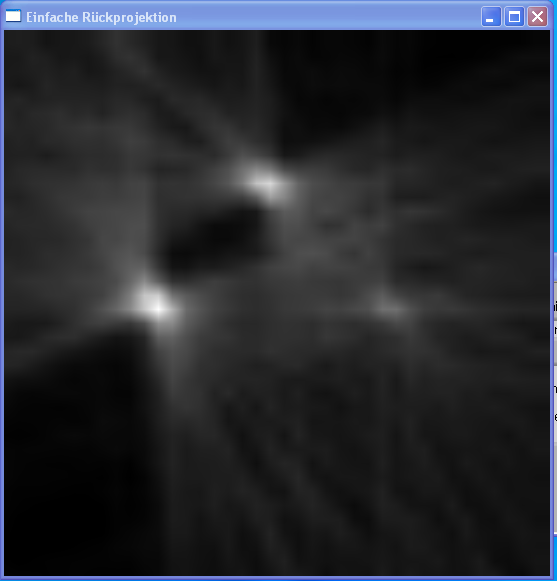
\includegraphics[width=0.3\textwidth, height=0.2\textheight]{pic/Einzelfenster_Bilder/unbekannte_Quelle/unbek4einf_prj.png}
                & 
                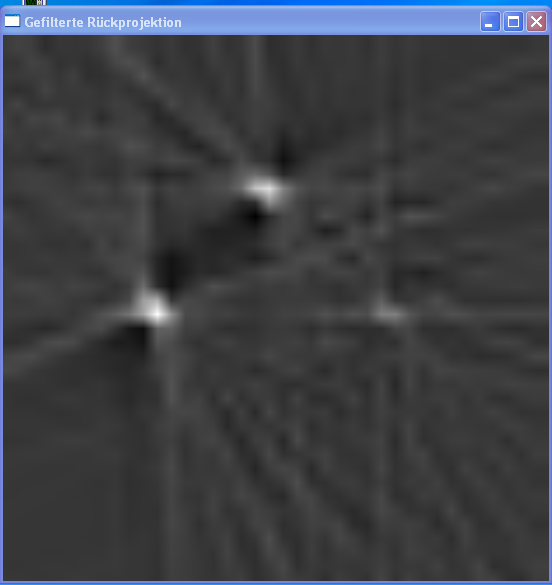
\includegraphics[width=.3\textwidth, height=0.2\textheight]{pic/Einzelfenster_Bilder/unbekannte_Quelle/unbek4gef_prj.png} \pagebreak
            \end{tabular}
            \end{center}
            \captionof{figure}{Screenshots der Bildenstehung der gefilterten (rechts) und ungefilterten (links) Rückprojektion}
          \minipend\\ \ \\
            \textbf{Untersuchung des Einflusses verschiedener Filter}\\
          \minipanf  
              \begin{tabular}{p{4.5cm}p{4.5cm}p{4.5cm}c}
                  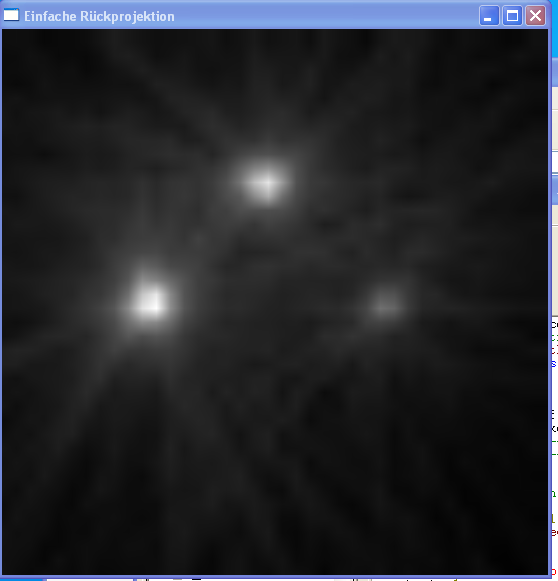
\includegraphics[width=0.25\textwidth, height=0.15\textheight]{pic/Einzelfenster_Bilder/unbekannte_Quelle/unbek5_einf_prj.png}
                  \captionof{figure}{ungefilterten Rückprojektion}
                  & 
                  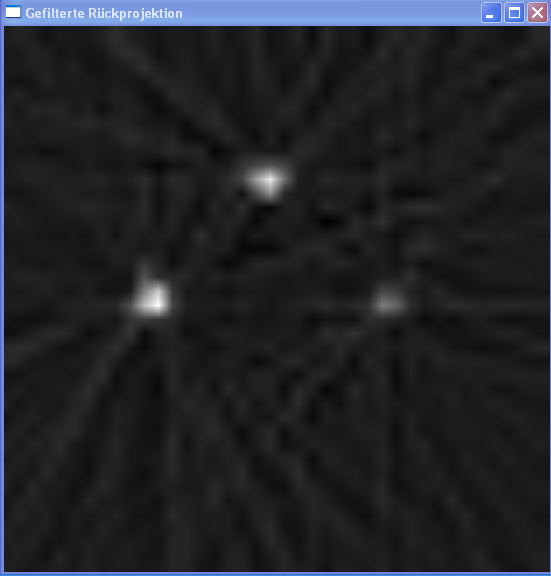
\includegraphics[width=.25\textwidth, height=0.15\textheight]{pic/Einzelfenster_Bilder/unbekannte_Quelle/unbek5_ramp.png}
                  \captionof{figure}{Rampf-Filter}
                  &
                  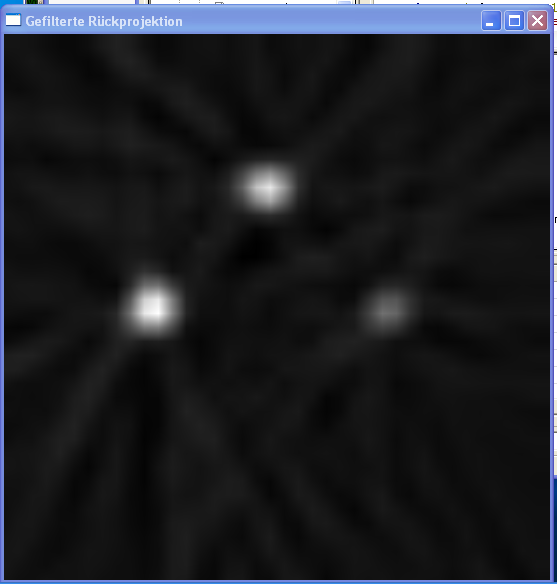
\includegraphics[width=0.25\textwidth, height=0.15\textheight]{pic/Einzelfenster_Bilder/unbekannte_Quelle/unbek5_hanning_weighted.png}
                  \captionof{figure}{Hanning-weighted-Filter}\\
                  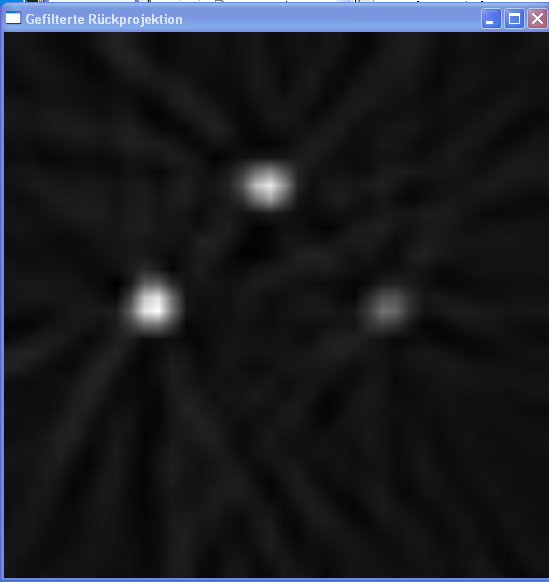
\includegraphics[width=.25\textwidth, height=0.15\textheight]{pic/Einzelfenster_Bilder/unbekannte_Quelle/unbek5_middle.png} 
                  \captionof{figure}{Middle-Filter}
                  &
                  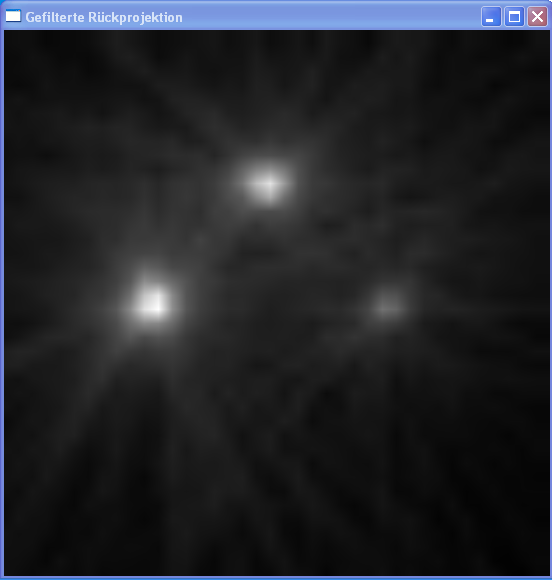
\includegraphics[width=0.25\textwidth, height=0.15\textheight]{pic/Einzelfenster_Bilder/unbekannte_Quelle/unbek5_rausch3.png}
                  \captionof{figure}{Rauschfilter bei Dimension 3}
                  & 
                  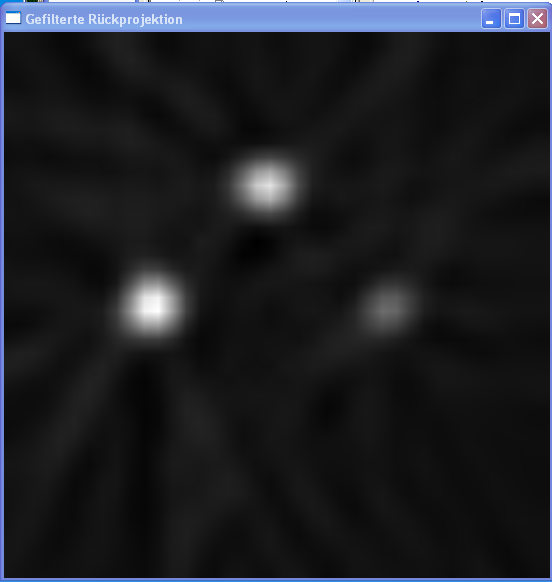
\includegraphics[width=.25\textwidth, height=0.15\textheight]{pic/Einzelfenster_Bilder/unbekannte_Quelle/unbek5_rausch13.png}               
                  \captionof{figure}{Rauschfilter bei Dimension 13} \pagebreak[2] 
                  \\
                  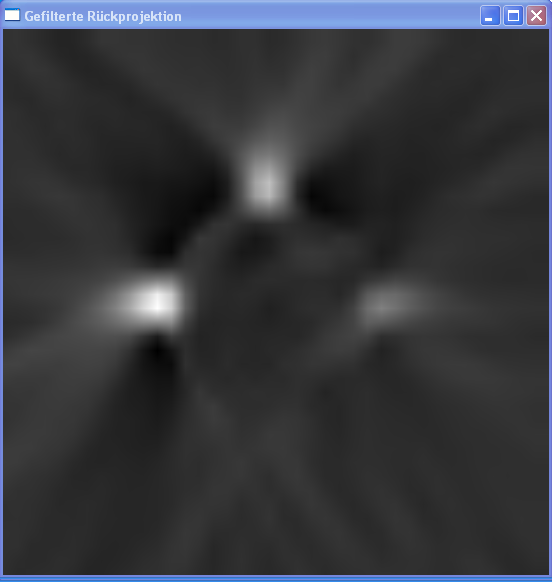
\includegraphics[width=0.25\textwidth, height=0.15\textheight]{pic/Einzelfenster_Bilder/unbekannte_Quelle/unbek5_rausch25.png}
                  \captionof{figure}{Rauschfilter bei Dimension 25}
                  &
                  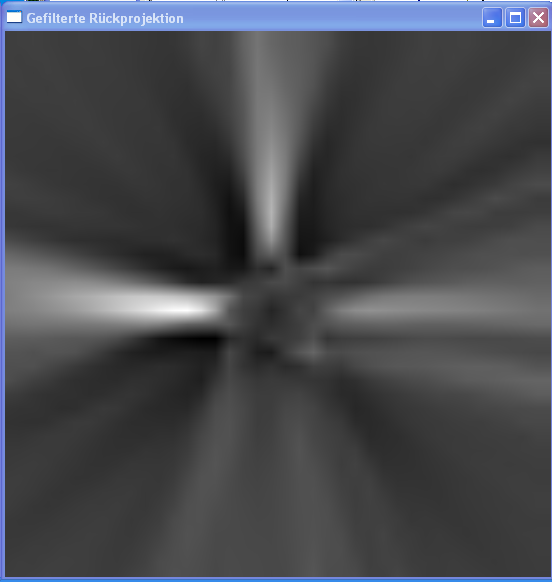
\includegraphics[width=.25\textwidth, height=0.15\textheight]{pic/Einzelfenster_Bilder/unbekannte_Quelle/unbek5_rausch36.png} 
                  \captionof{figure}{Rauschfilter bei Dimension 36}
                  &
                  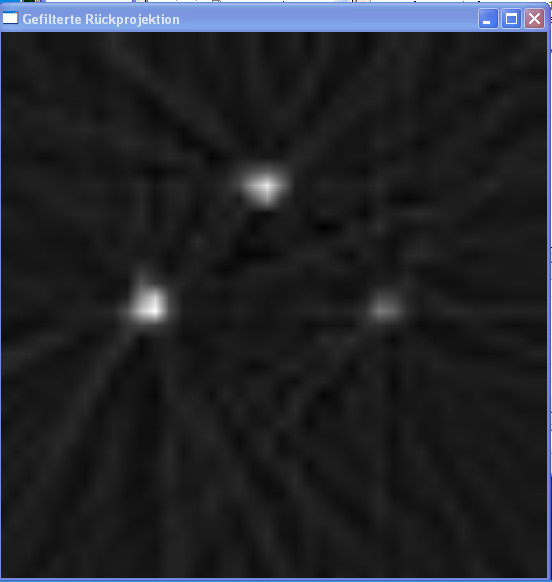
\includegraphics[width=.25\textwidth, height=0.15\textheight]{pic/Einzelfenster_Bilder/unbekannte_Quelle/unbek5_shepp-logan.png}
                  \captionof{figure}{Shepp-Logan-Filter}
                \end{tabular}
                Die Abbildungen drei bis elf zeigen die Anwendung verschiedener Filter auf die ungefilterte Rückprojektion, wobei der Standardwert der Dimension 13 ist
            
            \minipend\\ \ \\            
            
            
        \subsubsection{Messung mit einer Punktquelle, Phantom an-/insotroper Dichteverteilung}